\makechapter{Result}{Result}{Result\label{result}}

The following is a description of the implementation and results of a set of
experiments run in order to implement the clock synchronisation functionality
defined by the USB Audio Class specification.

The code for these experiments, along with the results of the measurements, can
be found at the USB Audio Experimets repository made for this project
\cite{github:usbAudioExperiments}. These are grouped by tags, which refers to
the version of the code used during that particular experiment.

\section{Experiment 1}

The first step of getting clock synchronisation to work, was to figure
out a way to measure the current rate of data sent to the USB device.

A Nucleo-F411RE devboard was used to mock up a USB audio card. 

\todo{Add theory on devboards. Include info on gpios and their
alternate functions}
\todo{Add theory on the different STM32 devboards discussed}

This board can be configured as a Full Speed USB device, which enables a
bandwidth of up to 12 Mbit/s. This is enough bandwidth to transmit two
channels of audio at a sampling rate of 48 kHz.

The goal of experiment 1 was to set up a USB audio class device, and
for each USB interrupt to this device toggle a \acrshort{gpio} pin.
This pin was then connected to a Saleae logic analyzer, which could
record the rate this pin changed.

The changes of the states of these pins where recorded with the logic
analyzer. These recordings where parsed into a diagram of the rate of
interrupts over time, using a python script included in the USB Audio
Experiments repository \cite{github:usbAudioExperiments}.

\begin{figure}[h]
	\caption{Rate over time for experiment 1}
	\centering
	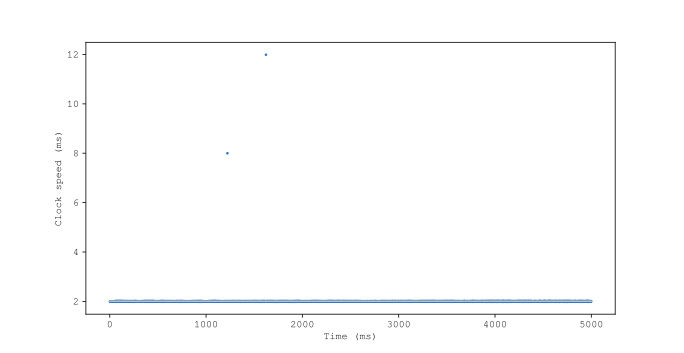
\includegraphics[width=0.8\textwidth]{Experiment-1/Experiment-1.png}
	\label{fig:experiment-1}
\end{figure}

Figure \ref{fig:experiment-1} shows the result for this experiment.
The result is a rate of one USB request every two milliseconds. There
is however two outliers, where one request took eight milliseconds,
and one twelve milliseconds. Figure \ref{fig:experiment-1-raw}
displays Saleaes analyzer software Logic. This includes the normal
rates at about two milliseconds each, and one of the outliers where
packets seems to have been dropped

\begin{figure}[h]
	\caption{A piece of the captured data for experiment 1, in Saleaes
	analyzer software Logic.}
	\centering
	\includegraphics[width=0.8\textwidth]{Experiment-1/Experiment-1-raw.png}
	\label{fig:experiment-1-raw}
\end{figure}

The reason for these outliers might have been caused by the choice of
the USB hosts operating system, which was Ubuntu. It could also depend
on the fact that the host computer acted both as a USB host for the
audio output, the devboard programmer and the logic analyzer at the
same time, which might have limited the bandwidth available for the
audio device, and therefore dropping USB messages. Another cause could
have been that the USB connection between the host machine and the
mocked up audio card was made using patch cables, with an unspecified
impedance, resulting in an unstable USB connection.

\section{Experiment 1.1}

The next step was to gather more extensive data about the USB
transmissions, in order to narrow down the problems in experiment 1.
For this experiment, two different \acrshort{gpio} pins where used to
flag for two different states. The first one was set to toggle each
time the device triggered a general USB interrupt. When this interrupt
occurred, the device parsed the USB request and checked if it
contained a buffer with audio samples. If this was the case, it
toggled the second pin.

In order to measure the size of the data packets sent from the host
during each transmission, a USART output was included in the mocked
device program. Each time the device receives an interrupt containing
audio data, it measures the length of this data packet, and write it
to the UART output. This was then captured by the logic analyzer, and
parsed along with the rest of the measured data with the python
parser.

\todo{Explain USART}

For the UART to have time to write the length of each packet before
the next one arrived, it would need to output at a rate much higher
then the rate of USB messages. Experiment 1 showed that the rate of
the USB data transmitted from the host machine was around once every
two milliseconds, which results in 500 transmissions each second.
Using a sufficiently high UART rate, in this case 115200 bits/s, it
could be ensured that the UART would be able to output a sufficiently
large amount of bytes between each interrupt. 

\todo{Rewrite this so it makes sense}

Adding these extra signals resulting in the measurement in figure
\ref{fig:experiment-1-1-raw}. The outliers still remains, as can be
seen in the large pulse in the middle. But now it can be observed that
each of the interrupts seems to correspond to a valid audio packet, as
the rate of both pins are about the same. 

\begin{figure}[h]
	\caption{A piece of the captured data for experiment 1.1, in Saleaes
	analyzer software Logic.}
	\centering
	\includegraphics[width=0.8\textwidth]{Experiment-1/Experiment-1-1-raw.png}
	\label{fig:experiment-1-1-raw}
\end{figure}

The third reading is the serial output from the device. The large
headroom between the end of these transmissions to the next interrupt
indicates that the rate for the USART is high enough to not cause any
problems regarding timing. In figure \ref{fig:experiment-1-1-serial},
the message containing the length of a USB requests audio buffer is
shown to be 288 bytes long.

\begin{figure}[h]
	\caption{A zoomed in piece of the captured data for experiment
	1.1, showing the USART message being sent.}
	\centering
	\includegraphics[width=0.8\textwidth]{Experiment-1/Experiment-1-1-serial.png}
	\label{fig:experiment-1-1-serial}
\end{figure}

Using the python parser resulted in the diagrams shown in figure
\ref{fig:experiment-1-1}. Here the outliers can still be observed. But
along with the interrupt rate, the length of the USB requests audio
buffer is shown to be at a steady length of 288 bytes/message.

\begin{figure}[h]
	\caption{Rate over time and buffer length over time respectively
	for experiment 1.1}
	\centering
	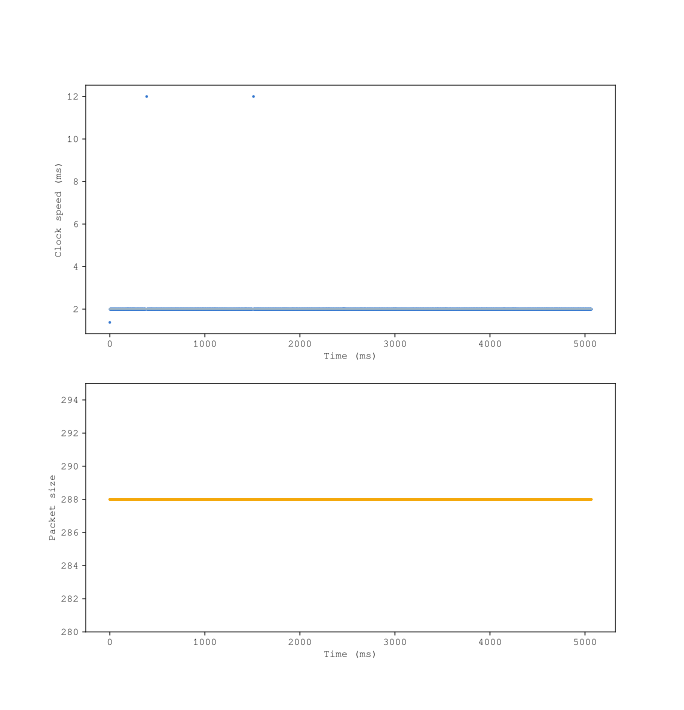
\includegraphics[width=0.8\textwidth]{Experiment-1/Experiment-1-1.png}
	\label{fig:experiment-1-1}
\end{figure}

\section{Experiment 1.2}

In order to eliminate some of these potential problems during
experiment 1 and 1.1, resulting in the outliers, the next attempt was
made using a separate computer acting as a USB host for the audio
device. This host used the Arch based operating system Manjaro.

Figure \ref{fig:experiment-1-2} shows the result of using this
separate host for the audio communication, and the previous host only
for the programmer and the logic analyzer. Now the outliers are all
gone, and left is a rate of about two milliseconds with a very minor
deviation. The packet sizes are still all 288 bytes long.

\begin{figure}[h]
	\caption{Rate over time and buffer length over time respectively
	for experiment 1.2}
	\centering
	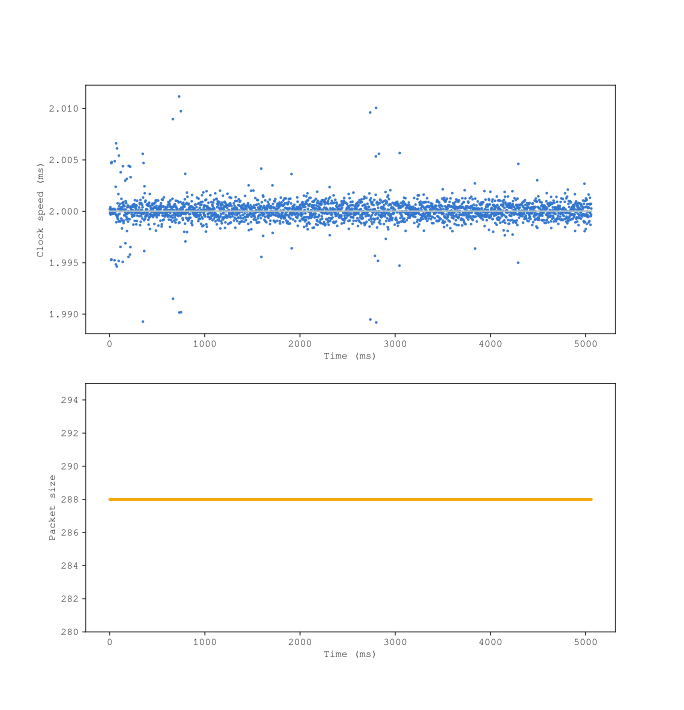
\includegraphics[width=0.8\textwidth]{Experiment-1/Experiment-1-2.png}
	\label{fig:experiment-1-2}
\end{figure}

The experiments 1, 1.1 and 1.2 shows that a rate of USB packets and
the size of the data contained in them can be measured. This is
measured with a low deviation in time, meaning that any change in rate
would be easily observed.

The next step is to try to make a request to the audio host for a
higher audio rate. The goal is to measure the size of each packet
increasing, as the host increases this rate.

